\documentclass[10pt]{article}
\usepackage[usenames]{color} %used for font color
\usepackage{amssymb} %maths
\usepackage{amsmath} %maths
\usepackage[utf8]{inputenc} %useful to type directly diacritic characters
\usepackage[letterpaper, portrait, margin=1in]{geometry}
\usepackage{graphicx,wrapfig}
\begin{document}
\subsection*{MSDS610 Week 5 Pig Assignment - Nathan Worsham}
Similar to previous weeks, I began this assignment by powering up my week 1 VM and then geting the download and unpacking the archive. And again similar to previous weeks I installed Pig into the home directory of my hadoop user, created a symbolic link, updated the environment variables for Pig, and then ran the test command successfully that the instructions called for. 
\par
\raisebox{-.6\height}{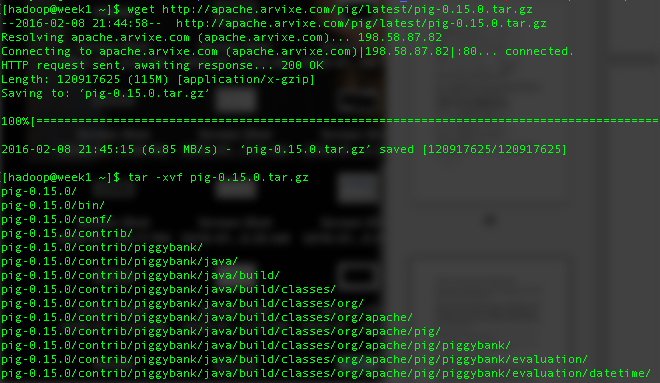
\includegraphics[width=8cm]{pig_wget.png}}%
\hfill
\raisebox{-.6\height}{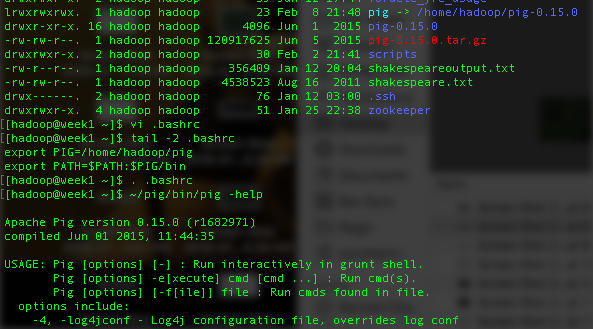
\includegraphics[width=8cm]{env_help.png}}%
\par
I went ahead and copied the interactive mode example with the \verb|/etc/passwd| file in local mode just to confirm it was working as expected. It did work as expected with the exception that it had some warnings of deprecated features.
\par
\raisebox{-.6\height}{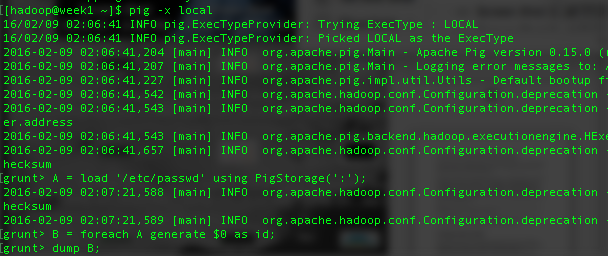
\includegraphics[width=9cm]{pig_local1.png}}%
\hfill
\raisebox{-.6\height}{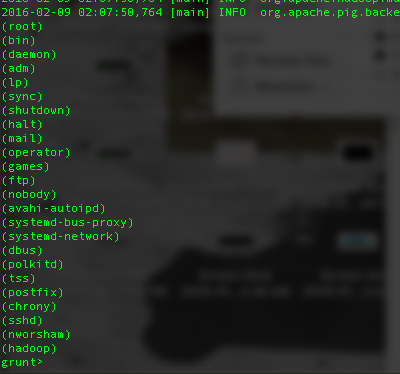
\includegraphics[width=7cm]{pig_local2.png}}%
\par
Next I wanted to do the exact same test but in Hadoop. Looking at the hadoop exercise, there needs to be an environment variable set for \verb|PIG_CLASSPATH| which it gives an example as "/mycluster/conf". I went ahead and looked for a conf directory at the root of the hadoop install but could find no such folder, so then I used the find command. None of the results seemed right and after carefully reading I noticed the instructions state "the directory that contains the core-site.xml". So re-running my find command targeting the core-site.xml--a file I was definitely familiar with from past weeks--I found the directory was hadoop/etc/hadoop. So I set my environment variable accordingly.
\begin{figure}[!h]
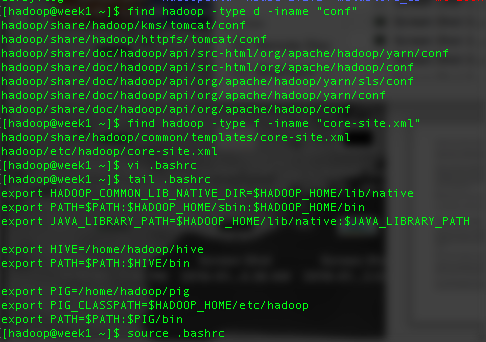
\includegraphics[scale=0.37]{env.png}
\centering
\end{figure}\\
\indent Now I started up HDFS and yarn then ran just simply \verb|pig| since the default mode is mapreduce mode. It started up with again the previous deprecation warnings. I was pleasantly surprised to learn that pig retains a command history that I could access with the up and down arrows from my keyboard. I was equally as pleased that running the same commands in mapreduce mode returned the same output, except that the return took a little longer.
\par
\raisebox{-.6\height}{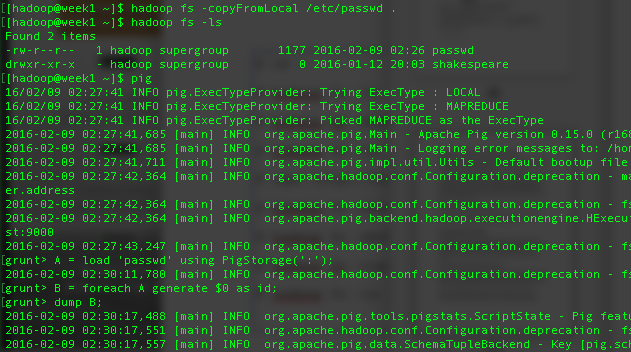
\includegraphics[width=8cm]{map1.png}}%
\hfill
\raisebox{-.6\height}{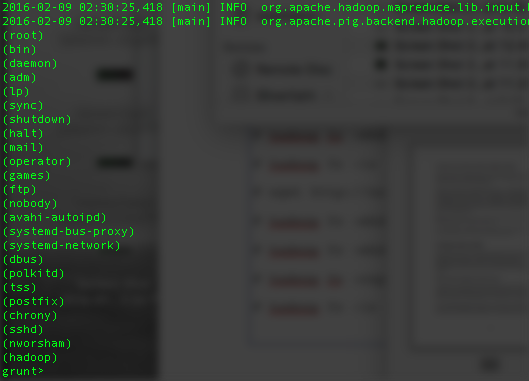
\includegraphics[width=8cm]{map2.png}}%
\par
I decided the next step would be good to do the pig tutorial for local and mapreduce mode. The first instruction was to make sure that \verb|JAVA_HOME| was set, which I checked and it was, but then it also asked for another environment variable--\verb|PIG_HOME|--to be set to the same as the previous environment variable \verb|PIG| which I went ahead and did. Next I needed to run the "ant" command in the tutorial directory, a command I had never heard of. I had to install the command first, looks like from its description it is a "Build tool for java". However after running the command, I did not receive the expected output, I received a couple of errors.
\begin{verbatim}
[echo]  *** Compiling Tutorial files ***
    [javac] /home/hadoop/pig-0.15.0/tutorial/build.xml:66: warning: 'includeantruntime' 
    was not set, defaulting to build.sysclasspath=last; set to false for repeatable builds
    [javac] Compiling 7 source files to /home/hadoop/pig-0.15.0/tutorial/build/classes

BUILD FAILED
/home/hadoop/pig-0.15.0/tutorial/build.xml:66: /home/hadoop/pig-0.15.0/build/ivy/lib/
Pig does not exist.
\end{verbatim}
I was able to fix the includeanttime warning by following a Stackoverflow.com (2011) thread and adding \verb|includeantruntime="false"| inside of the \verb|<javac>| options. The final error though was about a build directory not existing at the root level of pig. Taking a look at that area, indeed I saw no build directory but I did see a "build.xml" file just like there was in the tutorial directory. Given this info I assumed I would first need to run \verb|ant| at the root level but was a bit worried that might break something as the installation of pig I chose was the already built version and not the source. I went ahead and copied the entire pig directory to a test directory and ran the \verb|ant| command on the test instance. Sure enough it built the missing directories and running \verb|ant| inside of the tutorial directory now worked and I now had my pigtutorial.tar.gz file. 
\pagebreak
\begin{figure}[!h]
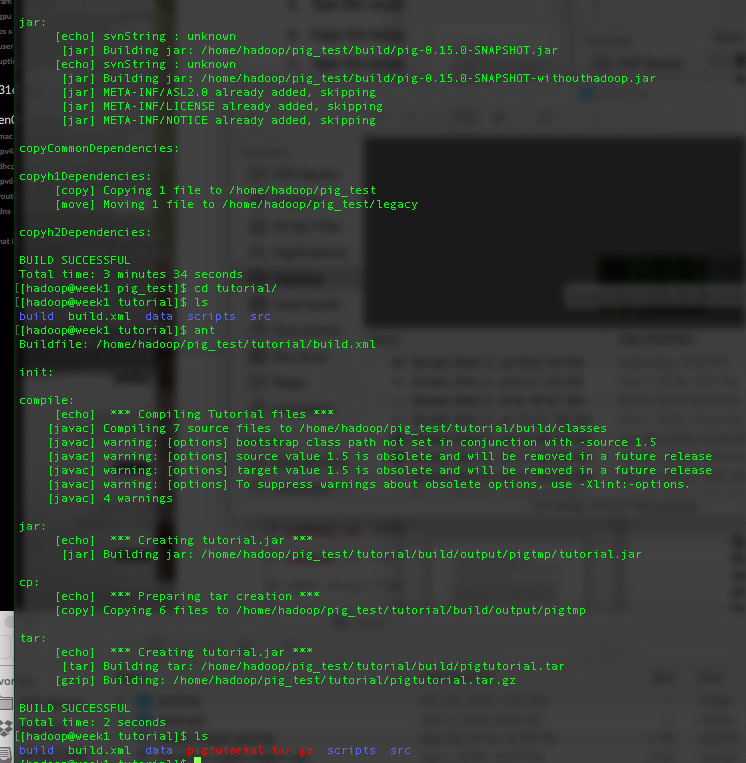
\includegraphics[scale=0.37]{ant_good.png}
\centering
\end{figure}\\
\indent After extracting the tar file, I had the remaining files I needed. First running the local test--\verb|script1-local.pig|--which appears to read the "excite-small.log", a log file of the Excite search engine and find the popular query phrases as they relate to times of the day. However the output from the local mode ended up with only single popular words, not phrases, and it seems to include stop words that probably should have been filtered out to make a better analysis but regardless shows the ability of the pig system.
\par
\raisebox{-.6\height}{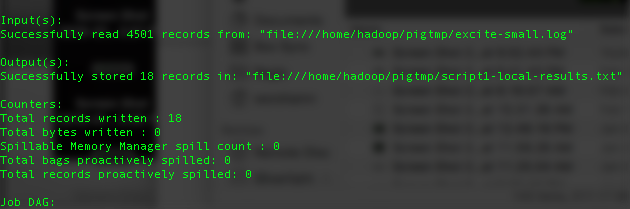
\includegraphics[width=8cm]{script1_results.png}}%
\hfill
\raisebox{-.6\height}{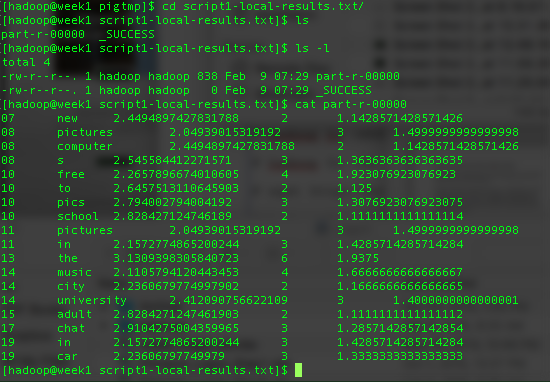
\includegraphics[width=8cm]{script1_success.png}}%
\par
Next I could try the mapreduce version of the excercise. I started by copying a \verb|bz2| version of the log file to the HDFS. Looking at the size of the file compared to the local version, it is considerably bigger--10 mb versus 204 kb. I had already taken care of the environment variable \verb|PIG_CLASSPATH| but now I needed to make \verb|HADOOP_CONF_DIR| equivallent to the same path.
\par
\raisebox{-.6\height}{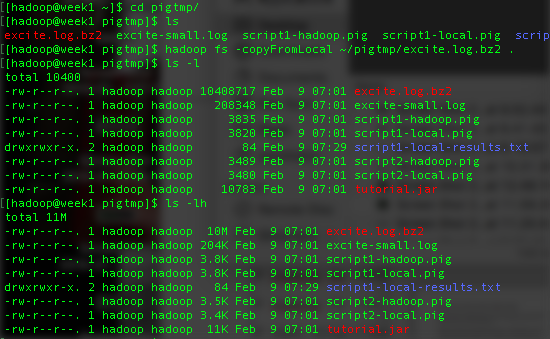
\includegraphics[width=8cm]{copy_log.png}}%
\hfill
\raisebox{-.6\height}{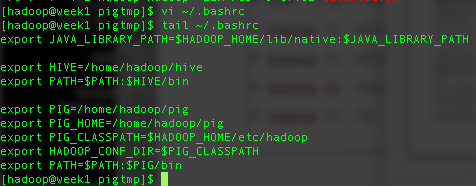
\includegraphics[width=8cm]{conf_dir.png}}%
\par
I was now ready to run the mapreduce version of the script. As expected it took considerably longer considering the much bigger file to analyze and also being within the HDFS.
\begin{figure}[!h]
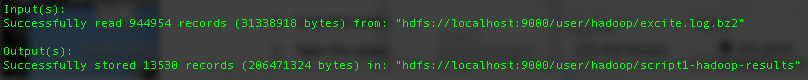
\includegraphics[scale=0.37]{hadoop_output1.png}
\centering
\end{figure}\\
\indent The results where much bigger than the local script test--13530 lines versus 18--and this time did have phrases in addition to single words. The results seemed to cover all hours of the day.
\begin{figure}[!h]
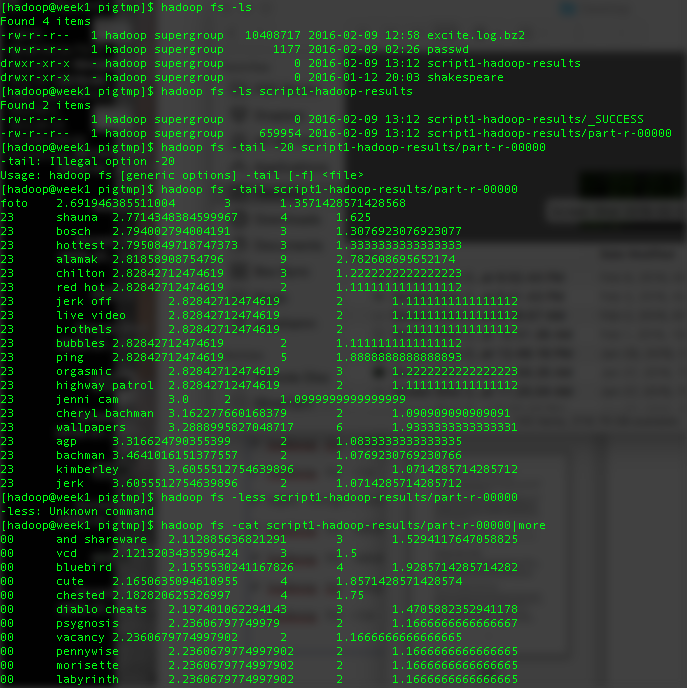
\includegraphics[scale=0.37]{hadoop_output2.png}
\centering
\end{figure}\\
\indent Furthermore it is interesting to compare the results at different hours of the day, example the noon hour ngram results seem to be "cleaner" than the 11 and 12 am results.
\pagebreak
\begin{figure}[!h]
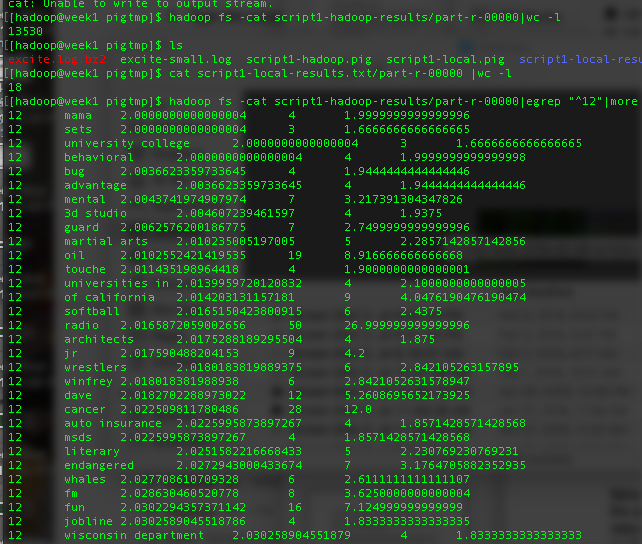
\includegraphics[scale=0.37]{noon.png}
\centering
\end{figure}\\
\indent Looking through the script1-hadoop.pig script, at first it would seem that "pig latin" is its own language but the more I look through the script the more I see that that the UDFs (user defined funchtions) are really where the heavy lifting is done. Looking into what exactly a UDF is, looks like it is a way to provide pig with custom processing and can be written in Java, JavaScript, Python, or Ruby (pig.apache.org, 2012). This made me think, why don't users then share the functions they have written but looks like pig has that as well, called piggybank. Currenlty piggybank only supports Java written functions. Pig latin looks like it is pretty in-depth but the fact that the script had to use a UDF to simply make the field lowercase--\verb|org.apache.pig.tutorial.ToLower(query)|--makes it seem like it is missing some pretty basic built-in functions. \\
\indent Not sure if the assignment required me to do the second set of scripts but out of interest I ran them. Again the local script only had minimal results, 3 versus 5343 for the hadoop script. This time the output was ngrams and their occurrence at the midnight hour and then the noon hour so you can see the difference. 
\par
\raisebox{-.5\height}{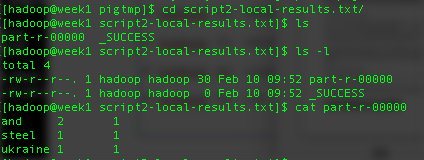
\includegraphics[width=8cm]{local2.png}}%
\hfill
\raisebox{-.5\height}{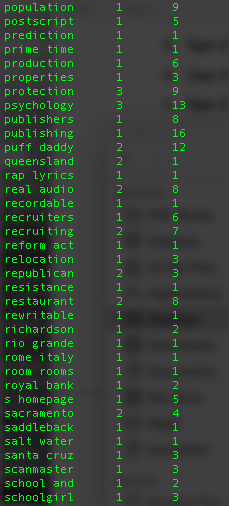
\includegraphics[width=4cm]{hadoop2.png}}%
\par
\subsection*{References}
pig.apache.org, 2016. Retrieved from http://pig.apache.org/docs/r0.14.0/start.html\\
Stackoverflow.com, 2011. Retrieve from http://stackoverflow.com/questions/5103384/ant-warning-includeantruntime-was-not-set\\
pig.apache.org, 2016. Retrieved from https://pig.apache.org/docs/r0.10.0/udf.html\#piggybank
\end{document}
